% Options for packages loaded elsewhere
\PassOptionsToPackage{unicode}{hyperref}
\PassOptionsToPackage{hyphens}{url}
\PassOptionsToPackage{dvipsnames,svgnames,x11names}{xcolor}
%
\documentclass[
  letterpaper,
  DIV=11,
  numbers=noendperiod]{scrartcl}

\usepackage{amsmath,amssymb}
\usepackage{iftex}
\ifPDFTeX
  \usepackage[T1]{fontenc}
  \usepackage[utf8]{inputenc}
  \usepackage{textcomp} % provide euro and other symbols
\else % if luatex or xetex
  \usepackage{unicode-math}
  \defaultfontfeatures{Scale=MatchLowercase}
  \defaultfontfeatures[\rmfamily]{Ligatures=TeX,Scale=1}
\fi
\usepackage{lmodern}
\ifPDFTeX\else  
    % xetex/luatex font selection
\fi
% Use upquote if available, for straight quotes in verbatim environments
\IfFileExists{upquote.sty}{\usepackage{upquote}}{}
\IfFileExists{microtype.sty}{% use microtype if available
  \usepackage[]{microtype}
  \UseMicrotypeSet[protrusion]{basicmath} % disable protrusion for tt fonts
}{}
\makeatletter
\@ifundefined{KOMAClassName}{% if non-KOMA class
  \IfFileExists{parskip.sty}{%
    \usepackage{parskip}
  }{% else
    \setlength{\parindent}{0pt}
    \setlength{\parskip}{6pt plus 2pt minus 1pt}}
}{% if KOMA class
  \KOMAoptions{parskip=half}}
\makeatother
\usepackage{xcolor}
\setlength{\emergencystretch}{3em} % prevent overfull lines
\setcounter{secnumdepth}{-\maxdimen} % remove section numbering
% Make \paragraph and \subparagraph free-standing
\makeatletter
\ifx\paragraph\undefined\else
  \let\oldparagraph\paragraph
  \renewcommand{\paragraph}{
    \@ifstar
      \xxxParagraphStar
      \xxxParagraphNoStar
  }
  \newcommand{\xxxParagraphStar}[1]{\oldparagraph*{#1}\mbox{}}
  \newcommand{\xxxParagraphNoStar}[1]{\oldparagraph{#1}\mbox{}}
\fi
\ifx\subparagraph\undefined\else
  \let\oldsubparagraph\subparagraph
  \renewcommand{\subparagraph}{
    \@ifstar
      \xxxSubParagraphStar
      \xxxSubParagraphNoStar
  }
  \newcommand{\xxxSubParagraphStar}[1]{\oldsubparagraph*{#1}\mbox{}}
  \newcommand{\xxxSubParagraphNoStar}[1]{\oldsubparagraph{#1}\mbox{}}
\fi
\makeatother


\providecommand{\tightlist}{%
  \setlength{\itemsep}{0pt}\setlength{\parskip}{0pt}}\usepackage{longtable,booktabs,array}
\usepackage{calc} % for calculating minipage widths
% Correct order of tables after \paragraph or \subparagraph
\usepackage{etoolbox}
\makeatletter
\patchcmd\longtable{\par}{\if@noskipsec\mbox{}\fi\par}{}{}
\makeatother
% Allow footnotes in longtable head/foot
\IfFileExists{footnotehyper.sty}{\usepackage{footnotehyper}}{\usepackage{footnote}}
\makesavenoteenv{longtable}
\usepackage{graphicx}
\makeatletter
\def\maxwidth{\ifdim\Gin@nat@width>\linewidth\linewidth\else\Gin@nat@width\fi}
\def\maxheight{\ifdim\Gin@nat@height>\textheight\textheight\else\Gin@nat@height\fi}
\makeatother
% Scale images if necessary, so that they will not overflow the page
% margins by default, and it is still possible to overwrite the defaults
% using explicit options in \includegraphics[width, height, ...]{}
\setkeys{Gin}{width=\maxwidth,height=\maxheight,keepaspectratio}
% Set default figure placement to htbp
\makeatletter
\def\fps@figure{htbp}
\makeatother

\KOMAoption{captions}{tableheading}
\makeatletter
\@ifpackageloaded{caption}{}{\usepackage{caption}}
\AtBeginDocument{%
\ifdefined\contentsname
  \renewcommand*\contentsname{Table of contents}
\else
  \newcommand\contentsname{Table of contents}
\fi
\ifdefined\listfigurename
  \renewcommand*\listfigurename{List of Figures}
\else
  \newcommand\listfigurename{List of Figures}
\fi
\ifdefined\listtablename
  \renewcommand*\listtablename{List of Tables}
\else
  \newcommand\listtablename{List of Tables}
\fi
\ifdefined\figurename
  \renewcommand*\figurename{Figure}
\else
  \newcommand\figurename{Figure}
\fi
\ifdefined\tablename
  \renewcommand*\tablename{Table}
\else
  \newcommand\tablename{Table}
\fi
}
\@ifpackageloaded{float}{}{\usepackage{float}}
\floatstyle{ruled}
\@ifundefined{c@chapter}{\newfloat{codelisting}{h}{lop}}{\newfloat{codelisting}{h}{lop}[chapter]}
\floatname{codelisting}{Listing}
\newcommand*\listoflistings{\listof{codelisting}{List of Listings}}
\makeatother
\makeatletter
\makeatother
\makeatletter
\@ifpackageloaded{caption}{}{\usepackage{caption}}
\@ifpackageloaded{subcaption}{}{\usepackage{subcaption}}
\makeatother
\ifLuaTeX
  \usepackage{selnolig}  % disable illegal ligatures
\fi
\usepackage{bookmark}

\IfFileExists{xurl.sty}{\usepackage{xurl}}{} % add URL line breaks if available
\urlstyle{same} % disable monospaced font for URLs
\hypersetup{
  pdftitle={Sequênciamento de teceira geração, PacBIO},
  colorlinks=true,
  linkcolor={blue},
  filecolor={Maroon},
  citecolor={Blue},
  urlcolor={Blue},
  pdfcreator={LaTeX via pandoc}}

\title{Sequênciamento de teceira geração, PacBIO}
\author{}
\date{2024-06-25}

\begin{document}
\maketitle

\section{Sequênciamento de terceira geração
PacBIO}\label{sequuxeanciamento-de-terceira-gerauxe7uxe3o-pacbio}

\begin{figure}[H]

{\centering \includegraphics{pacbio_files/mediabag/wEPv4PNBZ3i6gAAAABJR.png}

}

\caption{PacBio sequencing}

\end{figure}%

A tecnologia da pacbio se baseia em
\texttt{SMRT\ (Single-Molecule\ Real\ Time)} no qual é possiível
observar a adição de nucleotideos em tempo real, pois é usado uma enzima
modificada com alta afinidade por nucleotídeos floróforos, toda vez que
um nucleotídeo é adicionado a fita complementar é emitido luz do
floróforo expecífico. Tal como todos os tipos de sequênciamento de
terceira geração, suas vantagems é sequênciar fragmentos longos e não
necessita a etapa de amplificação por PCR

\begin{figure}[H]

{\centering 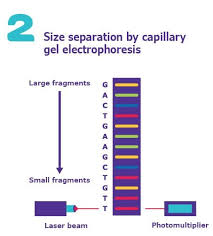
\includegraphics{pacbio_files/mediabag/Z.jpg}

}

\caption{SMRT}

\end{figure}%

\section{Preparo de biblioteca}\label{preparo-de-biblioteca}

está enzima fica presa a um poço, chamdos de
\texttt{ZMW\ (Zero-Mode\ Waveguide\ Detector)}. Este detector é
fundamental pois é a menor estrutura passível de suportar volume já
criada, e isso é fundamental para o funcionamento da tecnologia, a
detecção de volume é de 1 zeptolitro, ou um trilionesimo e milesimo de
litro. Na superfície do leitor, junto com o fragmento alvo, fragmento
este que tem a biblioteca de preparo circularizado o que aumenta a
eficiência da codificação, assim com ambas os sentidos das fitas de dna
sendo sequênciadas. além desta circularização é adicionado um barcode
para poder se possível indentificar a amostra.

\begin{figure}[H]

{\centering \includegraphics{pacbio_files/mediabag/yADUzqnwBu3VM0zM7xo3.png}

}

\caption{Preparo de biblioteca}

\end{figure}%

\section{Sequênciamento}\label{sequuxeanciamento}

Há emissão de luz do fundo pra cima do poço, mas por conta dos
\texttt{ZWMs} tere uma capacidade de volue muito pequena a luz emitida
não chega ao topo do poço, apenas ficando mais intença ao fundo dele.
Dentro da reação há, o fragmento preparado, a enzima que é forçada a
ficar no fundo do poço e os floróros modificados, eles possuem 5
fosfatos. quando a luz é emitida e só possível de detectar no fundo do
poço.

\begin{figure}[H]

{\centering \includegraphics{pacbio_files/mediabag/images-q=tbn-ANd9GcQ.jpg}

}

\caption{ZMW}

\end{figure}%

Existe um ruido de luz, uma florecência basal de todos os nucleotídeos
(bases as quais têm cores diferentes, relativa a cada base). Mas quando
a DNA polimeraze recruta a nucleotídeo molde para a fita complementar,
sua fluorecência é detectada por mais tempo permitindo assim um pico no
gráfico da detecção de florecência, e assim distinguindo cada base em
ordem

\begin{figure}[H]

{\centering \includegraphics{pacbio_files/mediabag/images-q=tbn-ANd9GcQ1.jpg}

}

\caption{Gráfico de florecência}

\end{figure}%

\section{Taxa de erro}\label{taxa-de-erro}

A tecnologia da PacBio possue uma alta taxa de erro, cerca de 5 a cada
100, ou \texttt{5\%}, isso é devido a alta velocidade de polimerização
da enzima, a mesma faz cerca de mil pares de bases por segundo e o
detector não consegue diferênciar todos os floróforos associados a cada
nucleotídeo. Porém, esses erros não vêm da característica do fragmento,
mas sim da tecnica. Ou seja, para fragmentos difíceis de sequênciar a
tecnologia da PacBio é mais interresante, já que os erros são
aleatórios, basta sequênciar o fragmento várias vezes para se ter uma
boa precisão. Mesmo para regiôes difíceis de sequênciar como telômeros e
centrômeros. Por isso que no preparo da biblioteca é adicionado
adaptadores a fim de circularizar o fragmento, para que em várias
rodadas cubram os floróforos associados as bases os quais não foram
diferenciados nas rodadas se sequênciamento anteriores. Aumentando assim
a eficácia de \texttt{99\%}. \textbf{Entretanto, para que isso ocorra é
necessário diminuir o tamanho do fragmento}



\end{document}
